\subsection{Grundlagen}
\begin{frame}{Minimalmaschine - ein idealisierter Prozessor}
	\only<1|handout:1>{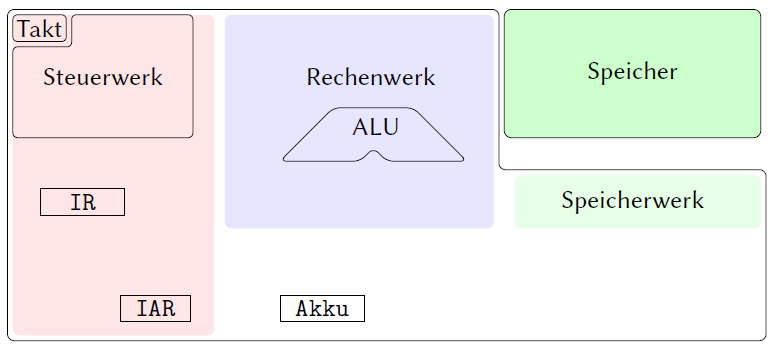
\includegraphics[width=\linewidth]{../topics/speicher-mima/MIMA_simple.png}} \only<2|handout:2>{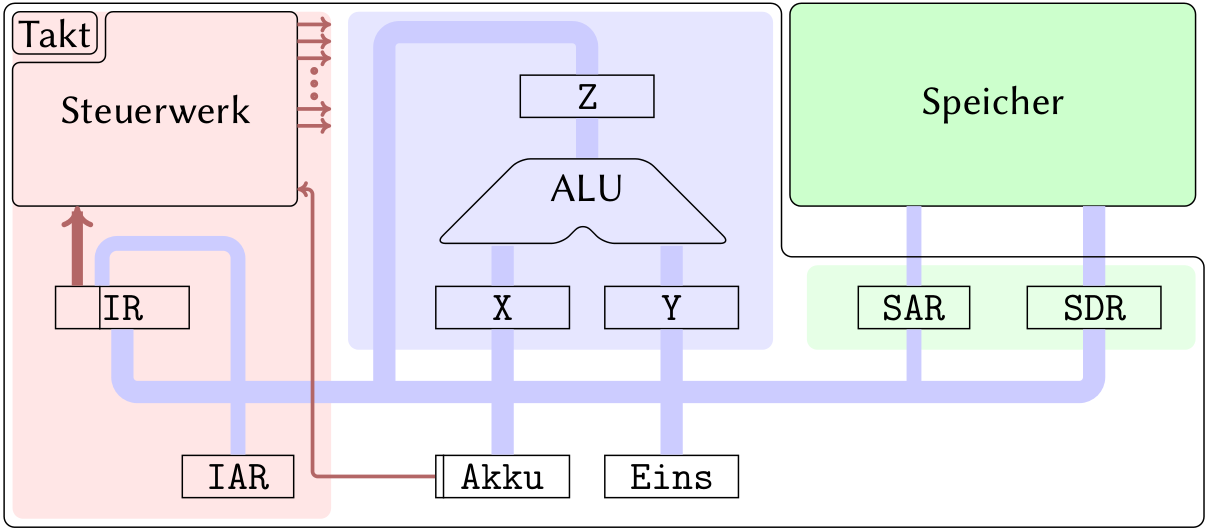
\includegraphics[width=\linewidth]{../topics/speicher-mima/MIMA.png}}
\end{frame}

\begin{frame}[plain]{Minimalmaschine: Befehle}\small
\begin{columns}
	\begin{column}{0.6\textwidth}
		\begin{tabular}{|l|l|}
			\toprule
				% Zugriffsoperationen
				LDC $c$ & $c \rightarrow Akku$ \\
				LDV $a$ & $M(a) \rightarrow Akku$ \\
				STV $a$ & $M(a) \leftarrow Akku$ \\
				LDIV $a$ & $M(M(a)) \rightarrow Akku$ \\
				STIV $a$ &$M(M(a)) \leftarrow Akku$ \\
				\midrule
				% Rechenoperationen
				ADD $a$ & $Akku + M(a) \rightarrow Akku$ \\
				AND $a$ & $Akku \ AND \ M(a) \rightarrow Akku$ \\
				OR $a$ & $Akku \ OR \ M(a) \rightarrow Akku$\\
				XOR $a$ & $Akku \ XOR \ M(a) \rightarrow Akku$\\
				NOT & Einskomplement von $Akku \rightarrow Akku$\\
				RAR & rotiert $Akku$ um 1 nach rechts $\rightarrow Akku$\\
				\midrule
				% Vergleichsoperationen
				EQL $a$ & $Akku \leftarrow \begin{cases}
											-1 & \text{, falls } Akku = M(a) \\
											0 & \text{, sonst} 
											\end{cases}$\\
				\midrule
				% Sprünge
				JMP $a$ & fahre fort mit Befehl an der Adresse $a$\\
				JMN $a$ & falls $Akku < 0$: JMP $a$\\
				HALT & stoppt die Mima\\
			\bottomrule	
		\end{tabular}
	\end{column}

	\begin{column}{0.32\textwidth}
		$c$: Konstante \\
		$a$: Adresse \\
		$M(a)$: Wert an Adresse $a$
	\end{column}
\end{columns}
\end{frame}

\begin{frame}{Minimalmaschine}
	\begin{exampleblock}{Eigenschaften}
		\begin{itemize}
		\item Adressen sind 20 Bit lang
		\item Werte sind 24 Bit lang
		\item Befehlscodierungen:
		\begin{itemize}
			\item 4 Bit für den OpCode und 20 Bit für einen Parameter (Adresse / Konstante)
			\item 8 Bit Befehl (Rest irrelevant)\\
			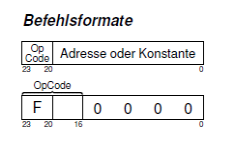
\includegraphics[width=100px]{../topics/speicher-mima/MIMA_Commands.png}\\
		\end{itemize} 
	\end{itemize}
	\end{exampleblock}
\end{frame}

\begin{frame}{Minimalmaschine}
	\begin{alertblock}{HALT}
		Jedes Programm muss mit HALT enden! Sonst läuft das Programm endlos weiter!
	\end{alertblock}

	\begin{alertblock}{Negative Konstanten}
		Negative Konstanten können nicht mit LDC geladen werden.\\
		Warum? \pause Unser Akku ist 24 Bit breit, aber wir können nur in die hinteren 20 Bit laden!
	\end{alertblock}
\end{frame}

\subsection{Aufgaben}
\begin{frame}{Minimalmaschine}
	\begin{exampleblock}{Aufgabe}
		Schreibe ein Programm, das eine an Adresse $a$ gegebene Zahl negiert und wieder in $a$ speichert. Die Adresse $R$ sei zum Zwischenspeichern frei verfügbar.
	\end{exampleblock}
	\pause
	\begin{block}{Lösung}
			LDV $a$\\
			NOT\\
			STV $R$\\
			LDC 1\\
			ADD $R$\\
			STV $a$\\
			HALT
		\end{block}
\end{frame}

\begin{frame}{}
	\begin{exampleblock}{Aufgabe}
		An den Adressen $a$ und $b$ liegen zwei ganze Zahlen in Zweierkomplementdarstellung. Schreibe ein Programm, das $M(a)-M(b)$ errechnet und das Ergebnis an Adresse $c$ speichert.
	\end{exampleblock}

	% \begin{block}{Lösung}
	% 	% TODO
	% \end{block}
\end{frame}

\begin{frame}{Minimalmaschine}
	\begin{exampleblock}{Aufgabe}
		Sei $n \in \nN_+$. Schreibe ein Programm, das eine an Speicheradresse $a_1$ gegebene, positive, ganze Zahl Modulo $n$ errechnet und an Adresse $a_2$ ablegt.
	\end{exampleblock}
\end{frame}

\begin{frame}{Minimalmaschine}
	\begin{block}{Lösung: Modulo $n$}\small
		start: LDC $n$\\
		$\qquad$ NOT\\
		$\qquad$ STV $R$\\
		$\qquad$ LDC 1\\
		$\qquad$ ADD $R$\\
		$\qquad$ STV $NEGN$\\
		$\qquad$ LDV $a_1$ \\
		\medskip
		while:   ADD $NEGN$\\
		$\qquad$ JMN ende\\
		$\qquad$ JMP while\\
		\medskip
		ende:    STV $LOOPRESULT$\\
		$\qquad$ LDC $n$\\
		$\qquad$ ADD $LOOPRESULT$\\
		$\qquad$ STV $a_2$\\
		$\qquad$ HALT\\
	\end{block}
\end{frame}

\begin{frame}{}
	\begin{exampleblock}{Aufgabe}
		Wie kann man das für $n=2$ besser, d.h. mit weniger Anweisungen, machen?
	\end{exampleblock}
\pause
	\begin{block}{Lösung: Modulo 2}
		start:   LDC 1 //000000000000000000000001 \\
		$\qquad$ AND $a_1$ \\
		$\qquad$ STV $a_2$ \\
		$\qquad$ HALT
	\end{block}
\end{frame}


	% \begin{block}{Lösung}
	% 	% TODO
	% \end{block}